\documentclass[12pt,letterpaper]{article}

\author{Jordan Bayles}
\title{Homework 4\\
\small ECE 478: Network Security}

%\date{}

%%Usepackage declarations
\usepackage[left=1in,top=1in,right=1in,bottom=1in]{geometry}
\usepackage{lastpage}
\usepackage{sectsty}
\usepackage{slashed}
\usepackage{amsmath}
\usepackage{amsfonts}
\usepackage{latexsym}
% Include for easy import of full pdf pages
\usepackage{pdfpages}
% Include for use of images
\usepackage{graphicx}
% Include for use of [H] placement specifier
\usepackage{float}
% Include for use of \toprule, \midrule, \bottomrule in tabular env.
\usepackage{booktabs}
% Include for setting spacing between lines
\usepackage{setspace}
% Code listing packages
\usepackage{listings}
\usepackage{xcolor}
\usepackage{color}
\usepackage[font=small,format=plain,labelfont=bf,up,textfont=it,up]{caption}

%% Package usages
\sectionfont{\normalsize}
\subsectionfont{\small}

%% New commands
\newcommand{\comment}[1]{}
\newcommand{\field}[1]{\mathbb{#1}} % requires amsfonts
\newcommand{\script}[1]{\mathcal{#1}} % requires amsfonts
\newcommand{\pd}[2]{\frac{\partial#1}{\partial#2}}

%% Access document variables
\makeatletter
\let\thetitle\@title
\let\theauthor\@author
\let\thedate\@date
\makeatother

%% Color Definitions
\definecolor{dkgreen}{rgb}{0,0.6,0}
\definecolor{gray}{rgb}{0.5,0.5,0.5}
\definecolor{mauve}{rgb}{0.58,0,0.82}
\definecolor{lightgrey}{gray}{0.8}
\definecolor{darkgrey}{gray}{1.6}

%% Code Listing Configuration
\DeclareCaptionFormat{listing}{\colorbox{gray}{\parbox{0.987\linewidth}{#1#2#3}}}
\captionsetup[lstlisting]{format=listing, labelfont=white, indention=0pt, textfont=white, margin=0pt, font={bf,footnotesize}, singlelinecheck=false}
\DeclareCaptionFont{white}{\color{white}}
\renewcommand{\lstlistingname}{Code}
\lstset{ %
  %Some lang opts: C++, C, Java, Python, Matlab, TeX, HTML, SQL, Verilog, VHDL, make, ...
  basicstyle=\footnotesize\ttfamily , % the size of the fonts that are used for the code
  numbers=left,                       % where to put the line-numbers
  numberstyle=\scriptsize\color{darkgray}, % the style that is used for the line-numbers
  stepnumber=2,                       % the step between two line-numbers. 
  numbersep=5pt,                      % how far the line-numbers are from the code
  backgroundcolor=\color{white},      % choose the background color. You must add \usepackage{color}
  showspaces=false,                   % show spaces adding particular underscores
  showstringspaces=false,             % underline spaces within strings
  showtabs=false,                     % show tabs within strings adding particular underscores
  frame=tb,                           % adds a frame around the code
  rulesepcolor=\color{gray},          % if not set, the frame-color may be changed on line-breaks within not-black text (e.g. commens (green here))
  tabsize=2,                          % sets default tabsize to 2 spaces
  captionpos=t,                       % sets the caption-position
  breaklines=true,                    % sets automatic line breaking
  breakatwhitespace=false,            % sets if automatic breaks should only happen at whitespace
  title=\lstname,                     % show the filename of files included with \lstinputlisting;
  keywordstyle=\color{blue},          % keyword style
  commentstyle=\color{dkgreen},       % comment style
  stringstyle=\color{mauve},          % string literal style
  escapeinside={\%*}{*)},             % if you want to add a comment within your code
  morekeywords={*,...}                % if you want to add more keywords to the set
  framexbottommargin=5pt,
}

\begin{document}
\begin{flushright}
\theauthor\\
\thedate
\end{flushright}
\begin{center}
\thetitle
\end{center}

\section*{0. Disclaimer}
\emph{This submission reflects my own understanding of the homework and
solutions. All of the ideas are my own, unless I explicitly acknowledge otherwise.}

\section*{1. Cookie contents and format}
The \verb~hashhw~ cookie has its value set to the username, creation timestamp,
and a hex encoded MAC generated
from the account name plus the timestamp ran through a md5 hash, truncated, and
then reran concatenated with a key
from a secret keyfile. Once a user enters the website while having a cookie,
the cookie is checked by utilizing the same username, timestamp, and key
to generate what the cookie value should be and then checking it to make sure
the MAC is valid.


\section*{2. Account token}
You completely control the username portion of the token, and can predict
the timestamp that will be associated with it.

\section*{3. Token contents for ADMIN access}
Must have the username set to ``admin,'' and the MAC address must match
the MAC generated by \verb~admin.<timestamp>~ using the key. The timestamp
doesn't really matter in and of itself.

\section*{4. MD5trunc collision yields ADMIN? How much effort?}
We know that the username must be admin, and we know that the mac must match
admin plus some timestamp, and must use the secret key only known to the server.
Thus, we must create a collision between \verb~admin.<some timestamp>~ and

\verb~ <some username != admin>.<some predicted or known timestamp>~. We can
make it a birthday attack instead of a brute force attack by using a list of
alternative usernames with known hashes, then calculating the MD5trunc of each
username to create a list of possible collisions to check against.

A naive attack is $2^n$ in complexity, but if we use a birthday kind of attack
instead of a second preimage, it makes the attack only $2^{n/2}$ in complexity.

It is important to note that we do NOT control the timestamp... it is a server
side variable. Thus we have two options for finding collsions: use a known
timestamp that occurs in the future (annoying, but what I chose to do), or
pregenerate a ton of MACs with known timestamps to make results less time
dependent (great for me, not so great for not hammering the server...)

\section*{5. MD5trunc collision and approach}
I found a collision using my python script, written to utilize the birthday
problem. Using a timestamp of \verb~090520140313~ and a maximum length of 4
for both the username and admin timestamp, I found that the following
values collide:
\begin{verbatim}
admin.1044        - 9bb5b59c8419244da574199300324198

fkkc.090520140313 - 9bb5b59c3433b0de8013e70d848ab799

Resulting MAC: cabe6ac811eb07a59e7cb30fd4597009
\end{verbatim}

\begin{figure}[H]
\centering
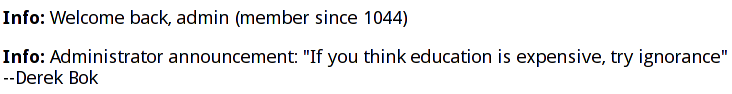
\includegraphics[width=5in]{admin4.png}
\end{figure}

\section*{6. Mechanics of the final attack}
The final attack used the collision above: at 03:13AM on May 9th, 2014, I created
a user with the username \verb~fkkc~ on the server. This created a cookie
with the MAC called ``Resulting MAC'' above, which I then modified to hold
the value \verb~admin.1044.cabe6ac811eb07a59e7cb30fd4597009~. A quick page
refresh resulted in the admin message:

\begin{verse}
"If you think education is expensive, try ignorance" --Derek Bok 
\end{verse}

\section*{7. Extension to different truncation lengths}
This type of attack is very sensitive to the length of the truncation utilized,
as it becomes increasingly difficult to match longer sections of the hash
sum. For example, using timestamps and usernames of both length $[1,4]$ results
in many instances of no collisions for a truncation of length 5, whereas
it has a very high probability of working for truncation of length 4. This set
of usernames, timestamps is quite large, resulting in
$26^4 * 10^4 = 4,569,760,000$ pairwise comparisons (using a linear traversal
on a finite array). For a length 5 truncation, to have a reliable chance of
success, we need to use timestamps and usernames of length 5 or more.

\begin{figure}[H]
\centering
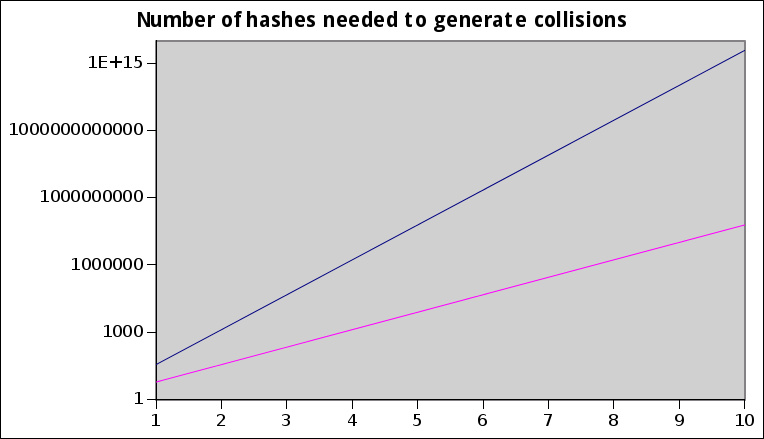
\includegraphics[width=5in]{complexity.png}
\caption{Number of hashes needed to generate a collision}
\end{figure}

\section*{Appendix}
\subsection{Collision finding script}
\lstinputlisting[language=Python]{collide.py}

\end{document}
